\documentclass{MFM-hw} % You must have the MFM-hw.cls file in your project or working directory (i.e. the same directory as this document) 

\HWauthor{Wei Qi}{226010267@link.cuhk.edu.cn} % Put your name and CUHK-SZ e-mail on this line
\HWno{2} % Enter the number of the homework you are working on
\HWcourse{MFM 5130} % Enter the course department and number here
\date{Oct 27, 2026}
\usepackage{amsmath}
\usepackage{amsfonts}
\usepackage{amssymb}
\usepackage{amsthm}
\usepackage{bm}
\usepackage{booktabs}
\usepackage{tikz}
\usetikzlibrary{calc,arrows.meta}
% \usepackage{hyperref}

\newcommand{\VaR}{\operatorname{VaR}}
\newcommand{\ES}{\operatorname{ES}}
\newcommand{\real}{\mathbb{R}}
\newcommand{\normal}{\operatorname{N}}
\newcommand{\N}{\mathcal{N}}
\newcommand{\dd}{\,\mathrm{d}}
\newcommand{\E}{\mathbb{E}}
\newcommand{\Par}{\operatorname{Par}}
\renewcommand{\P}{\mathbb{P}}
\newcommand{\Cov}{\operatorname{Cov}}
\newcommand{\Var}{\operatorname{Var}}
\newcommand{\Corr}{\operatorname{Corr}}
\newcommand{\tr}{\operatorname{tr}}
\newcommand{\rank}{\operatorname{rank}}
\newcommand{\diag}{\operatorname{diag}}
\newcommand{\inde}{\perp\!\!\!\perp}

% bold vectors and matrices
\newcommand{\bX}{\bm{X}}
\newcommand{\bY}{\bm{Y}}
\newcommand{\bZ}{\bm{Z}}
\newcommand{\bA}{\bm{A}}
\newcommand{\bB}{\bm{B}}
\newcommand{\bI}{\bm{I}}
\newcommand{\bS}{\bm{S}}
\newcommand{\bT}{\bm{T}}
\newcommand{\bL}{\bm{L}}
\newcommand{\bW}{\bm{W}}
\newcommand{\bx}{\bm{x}}
\newcommand{\by}{\bm{y}}
\newcommand{\bz}{\bm{z}}
\newcommand{\bs}{\bm{s}}
\newcommand{\bt}{\bm{t}}
\newcommand{\bu}{\bm{u}}
\newcommand{\bv}{\bm{v}}
\newcommand{\bw}{\bm{w}}
\newcommand{\ba}{\bm{a}}
\newcommand{\bb}{\bm{b}}
\newcommand{\be}{\bm{e}}
\newcommand{\bU}{\bm{U}}
\newcommand{\bV}{\bm{V}}
\newcommand{\bD}{\bm{D}}
\newcommand{\bO}{\bm{O}}
\newcommand{\bd}{\bm{d}}
\newcommand{\br}{\bm{r}}
\newcommand{\blambda}{\bm{\lambda}}
\newcommand{\bmu}{\bm{\mu}}
\newcommand{\bSigma}{\bm{\Sigma}}
\newcommand{\bLambda}{\bm{\Lambda}}
\newcommand{\bzero}{\bm{0}}
\newcommand{\bth}{\bm{\theta}}

\begin{document}
\maketitle

%=====================================================================
\HWproblem
\noindent\textit{(Multivariate normal distribution.)} $\bX=(X_1,\dots,X_d)$ has a multivariate normal distribution if
\[
    \bX \overset{d}{=} \bmu + \bA\bZ,
\]
where $\bZ=(Z_1,\dots,Z_k)^\top$, $Z_i\overset{\text{iid}}{\sim}\normal(0,1)$, $\bA\in\real^{d\times k}$, $\bmu\in\real^d$. Let $\bSigma=\bA\bA^\top$ and write $\bX\sim \normal_d(\bmu,\bSigma)$. Show that the characteristic function of $\bX$ is
\[
    \phi_{\bX}(\bt)=\E\Bigl[\exp\bigl(i\bt^\top\bX\bigr)\Bigr]
    =\exp\Bigl(i\bt^\top\bmu-\tfrac12\bt^\top\bSigma\bt\Bigr),\qquad \bt\in\real^d,
\]
based on the fact that $Z_1$ has density $f(x)=\exp(-x^2/2)/\sqrt{2\pi}$.

\medskip
\noindent\textbf{Solution.}

\smallskip
\noindent\textbf{Step 1 (the univariate factor).} We first compute the cf of a single standard normal variable. For $s\in\real$,
\begin{equation}\label{eq:univ}
    \E\bigl[e^{isZ_1}\bigr]
    =\frac{1}{\sqrt{2\pi}}\int_{\real} e^{isx-\frac{x^2}{2}}\dd x .
\end{equation}
Completing the square in the exponent,
\[
    isx-\frac{x^2}{2}=-\frac{(x-is)^2}{2}-\frac{s^2}{2},
\]
so that
\begin{equation}\label{eq:shift}
    \E\bigl[e^{isZ_1}\bigr]
    =e^{-\frac{s^2}{2}}\cdot\frac{1}{\sqrt{2\pi}}\int_{\real}e^{-\frac{(x-is)^2}{2}}\dd x .
\end{equation}
The shift of the contour from $\real$ to the horizontal line $\operatorname{Im}z=-s$ is legitimate: $z\mapsto e^{-z^2/2}$ is entire, and on the rectangle with vertices $\pm M$ and $\pm M-is$ one has, for $z=x+iy$ with $-s\le y\le 0$,
\[
    \bigl|e^{-z^2/2}\bigr| = e^{-\frac{x^2-y^2}{2}}\le e^{\frac{s^2}{2}}e^{-\frac{x^2}{2}},
\]
which is integrable in $x$ uniformly in $M$; hence by Cauchy's theorem the two vertical sides vanish as $M\to\infty$ and the integrals over the two horizontal lines coincide. Therefore the last integral equals $\int_{\real}e^{-u^2/2}\dd u=\sqrt{2\pi}$ and
\begin{equation}\label{eq:stdcf}
    \E\bigl[e^{isZ_1}\bigr]=e^{-\frac{s^2}{2}},\qquad s\in\real .
\end{equation}

\noindent\textbf{Step 2 (independence factorizes the cf).} Let $\bs=\bA^\top\bt\in\real^k$, so that $\bt^\top\bX=\bt^\top\bmu+\bt^\top\bA\bZ=\bt^\top\bmu+\bs^\top\bZ$. By the independence of $Z_1,\dots,Z_k$ and \eqref{eq:stdcf} applied to each coordinate with $s=s_j$,
\[
    \E\bigl[e^{i\bt^\top\bX}\bigr]
    =e^{i\bt^\top\bmu}\prod_{j=1}^{k}\E\bigl[e^{is_jZ_j}\bigr]
    =e^{i\bt^\top\bmu}\prod_{j=1}^{k}e^{-\frac{s_j^2}{2}}
    =e^{i\bt^\top\bmu}e^{-\frac{1}{2}\|\bs\|^2}.
\]

\noindent\textbf{Step 3 (identifying the quadratic form).} Since $\|\bs\|^2=\bs^\top\bs=\bt^\top\bA\bA^\top\bt=\bt^\top\bSigma\bt$,
\begin{equation}\label{eq:cfmvn}
    \boxed{\;\phi_{\bX}(\bt)=\exp\Bigl(i\bt^\top\bmu-\tfrac12\bt^\top\bSigma\bt\Bigr),\qquad \bt\in\real^d.\;}
\end{equation}
$\phi_{\bX}$ is continuous at $\bzero$ with $\phi_{\bX}(\bzero)=1$, so it is indeed a characteristic function. \qed

\smallskip
\noindent\textbf{Remark 1.1 (what \eqref{eq:cfmvn} really shows).} The computation nowhere uses a density of $\bX$; it uses only the representation and the univariate normal cf. Two consequences are worth recording.
\begin{enumerate}
    \item \emph{The law depends on $\bA$ only through $\bA\bA^\top$.} If $\bA_1\bA_1^\top=\bA_2\bA_2^\top=\bSigma$, then $\bmu+\bA_1\bZ$ and $\bmu+\bA_2\bZ'$ have the same cf and hence the same law (uniqueness of the characteristic function). This is exactly why the notation $\normal_d(\bmu,\bSigma)$ is unambiguous even though the factor $\bA$ is not unique (one may replace $\bA$ by $\bA Q$ for any orthogonal $Q\in\real^{k\times k}$).
    \item \emph{Existence for all positive semidefinite $\bSigma$.} $\bSigma=\bA\bA^\top$ is symmetric and $\bt^\top\bSigma\bt=\|\bA^\top\bt\|^2\ge0$; conversely every symmetric positive semidefinite $\bSigma$ admits such a factor (spectral decomposition $\bSigma=U\bLambda U^\top$ with $\bA=U\bLambda^{1/2}$). So $\normal_d(\bmu,\bSigma)$ is defined for every $\bmu\in\real^d$ and every positive semidefinite $\bSigma$, singular ones included.
\end{enumerate}

%=====================================================================
\HWproblem
\noindent\textit{(Conditional expectation.)} Let $\bX\sim\normal_d(\bmu,\bSigma)$. If
$\bSigma=\begin{pmatrix}\bSigma_{11}&\bSigma_{12}\\ \bSigma_{21}&\bSigma_{22}\end{pmatrix}$
is positive definite, show that
\[
    \bX_2\mid \bX_1=\bx_1\ \sim\ \normal_{d-k}\bigl(\bmu_{2.1},\bSigma_{22.1}\bigr),
\]
where
\[
    \bmu_{2.1}:=\bmu_2+\bSigma_{21}\bSigma_{11}^{-1}(\bx_1-\bmu_1),\qquad
    \bSigma_{22.1}:=\bSigma_{22}-\bSigma_{21}\bSigma_{11}^{-1}\bSigma_{12}.
\]

\medskip
\noindent\textbf{Solution.}

Write $\bX=(\bX_1,\bX_2)$ with $\bX_1\in\real^k$ and $\bX_2\in\real^{d-k}$, $\bmu=(\bmu_1,\bmu_2)$ accordingly. Throughout, $\bSigma_{11}$ denotes the $k\times k$ block; note that $\bSigma_{21}=\bSigma_{12}^\top$.

\smallskip
\noindent\textbf{Step 1 (the diagonalizing linear map).} Define the block-triangular matrix
\[
    \bT=\begin{pmatrix}\bI_k&\bzero\\ -\bSigma_{21}\bSigma_{11}^{-1}&\bI_{d-k}\end{pmatrix}\in\real^{d\times d},
    \qquad
    \bT\bX=\begin{pmatrix}\bX_1\\ \bX_2-\bSigma_{21}\bSigma_{11}^{-1}\bX_1\end{pmatrix}=:\begin{pmatrix}\bU\\ \bV\end{pmatrix}.
\]
Because $\bT\bX=\bT\bmu+(\bT\bA)\bZ$ with $\bT\bA\in\real^{d\times k}$ and $(\bT\bA)(\bT\bA)^\top=\bT\bSigma\bT^\top$, Problem 1 gives $\bT\bX\sim\normal_d\bigl(\bT\bmu,\bT\bSigma\bT^\top\bigr)$.

\smallskip
\noindent\textbf{Step 2 (block-diagonal covariance).} Using $\bSigma_{21}=\bSigma_{12}^\top$ and $\bSigma_{21}\bSigma_{11}^{-1}\bSigma_{11}=\bSigma_{21}$,
\[
    \bT\bSigma=\begin{pmatrix}\bSigma_{11}&\bSigma_{12}\\ -\bSigma_{21}\bSigma_{11}^{-1}\bSigma_{11}+\bSigma_{21}&-\bSigma_{21}\bSigma_{11}^{-1}\bSigma_{12}+\bSigma_{22}\end{pmatrix}
    =\begin{pmatrix}\bSigma_{11}&\bSigma_{12}\\ \bzero&\bSigma_{22.1}\end{pmatrix},
\]
and then, multiplying on the right by $\bT^\top=\begin{pmatrix}\bI_k&-\bSigma_{11}^{-1}\bSigma_{12}\\ \bzero&\bI_{d-k}\end{pmatrix}$ and using $\bSigma_{11}\bSigma_{11}^{-1}\bSigma_{12}=\bSigma_{12}$,
\[
    \bT\bSigma\bT^\top
    =\begin{pmatrix}\bSigma_{11}&\bSigma_{12}\\ \bzero&\bSigma_{22.1}\end{pmatrix}
     \begin{pmatrix}\bI_k&-\bSigma_{11}^{-1}\bSigma_{12}\\ \bzero&\bI_{d-k}\end{pmatrix}
    =\begin{pmatrix}\bSigma_{11}&\bzero\\ \bzero&\bSigma_{22.1}\end{pmatrix},
\]
because the upper-right block is $-\bSigma_{12}+\bSigma_{12}=\bzero$. Correspondingly,
\[
    \bT\bmu=\begin{pmatrix}\bmu_1\\ \bmu_2-\bSigma_{21}\bSigma_{11}^{-1}\bmu_1\end{pmatrix}=:\begin{pmatrix}\bmu_1\\ \bmu_{2\cdot1}\end{pmatrix} .
\]

\smallskip
\noindent\textbf{Step 3 (both blocks are nondegenerate).} Since $\bSigma$ is positive definite, so is $\bSigma_{11}$ (for $\ba\ne\bzero$, $(\ba,\bzero)^\top\bSigma(\ba,\bzero)=\ba^\top\bSigma_{11}\ba>0$), hence $\bSigma_{11}^{-1}$ exists. Moreover $\bSigma_{22.1}$ is positive definite: for $\bv\ne\bzero$, choosing $\bu=-\bSigma_{11}^{-1}\bSigma_{12}\bv$ gives
\[
    \begin{pmatrix}\bu\\ \bv\end{pmatrix}^\top\bSigma\begin{pmatrix}\bu\\ \bv\end{pmatrix}
    =\bv^\top\bigl(\bSigma_{22}-\bSigma_{21}\bSigma_{11}^{-1}\bSigma_{12}\bigr)\bv=\bv^\top\bSigma_{22.1}\bv>0,
\]
the inequality holding because $(\bu,\bv)\ne\bzero$. (This is the standard Schur-complement criterion: a symmetric block matrix is positive definite iff $\bSigma_{11}\succ0$ and $\bSigma_{22.1}\succ0$.)

\smallskip
\noindent\textbf{Step 4 ($\bU$ and $\bV$ are independent).} By Step 2 the transformed cf factorizes:
\[
    \phi_{(\bU,\bV)}(\bs,\br)
    =\exp\Bigl(i\bs^\top\bmu_1-\tfrac12\bs^\top\bSigma_{11}\bs\Bigr)
     \exp\Bigl(i\br^\top\bmu_{2\cdot1}-\tfrac12\br^\top\bSigma_{22.1}\br\Bigr)
    =\phi_{\bU}(\bs)\,\phi_{\bV}(\br),
\]
for all $(\bs,\br)$, which is precisely the cf of a pair of independent random vectors. Hence
\begin{equation}\label{eq:indep}
    \bU=\bX_1\ \inde\ \bV=\bX_2-\bSigma_{21}\bSigma_{11}^{-1}\bX_1,
    \qquad \bV\sim\normal_{d-k}\bigl(\bmu_{2\cdot1},\bSigma_{22.1}\bigr).
\end{equation}

\smallskip
\noindent\textbf{Step 5 (conditional law).} Let $h:\real^{d-k}\to\real$ be bounded and Borel. Because $\bX_2=\bV+\bSigma_{21}\bSigma_{11}^{-1}\bX_1$,
\[
    \E\bigl[h(\bX_2)\,\big|\,\bX_1\bigr]
    =\E\bigl[h\bigl(\bV+\bSigma_{21}\bSigma_{11}^{-1}\bX_1\bigr)\,\big|\,\bX_1\bigr]
    =\int_{\real^{d-k}} h\bigl(\bv+\bSigma_{21}\bSigma_{11}^{-1}\bX_1\bigr)\,f_{\bV}(\bv)\dd\bv
    =:g(\bX_1),
\]
where the second equality uses $\bV\inde\bX_1$ from \eqref{eq:indep} and $f_{\bV}$ is the $\normal_{d-k}(\bmu_{2\cdot1},\bSigma_{22.1})$ density. The right-hand side depends on $\bX_1$ only through the value $\bx_1$ taken by $\bX_1$, and the kernel
\[
    \nu(\bx_1,\cdot)=\normal_{d-k}\bigl(\bmu_{2\cdot1}+\bSigma_{21}\bSigma_{11}^{-1}\bx_1,\ \bSigma_{22.1}\bigr)
\]
satisfies $\int h\dd\nu(\bx_1,\cdot)=g(\bx_1)$; it is therefore a regular conditional distribution of $\bX_2$ given $\bX_1=\bx_1$. Since $\bmu_{2\cdot1}+\bSigma_{21}\bSigma_{11}^{-1}\bx_1=\bmu_2+\bSigma_{21}\bSigma_{11}^{-1}(\bx_1-\bmu_1)=\bmu_{2.1}$,
\begin{equation}\label{eq:cond}
    \boxed{\;\bX_2\mid\bX_1=\bx_1\ \sim\ \normal_{d-k}\bigl(\bmu_2+\bSigma_{21}\bSigma_{11}^{-1}(\bx_1-\bmu_1),\ \bSigma_{22}-\bSigma_{21}\bSigma_{11}^{-1}\bSigma_{12}\bigr).\;}
\end{equation}
\qed

\smallskip
\noindent\textbf{Remark 2.1 (density check).} The block inverse and determinant identities
\[
    \bSigma^{-1}=\begin{pmatrix}\bSigma_{11}^{-1}+\bSigma_{11}^{-1}\bSigma_{12}\bSigma_{22.1}^{-1}\bSigma_{21}\bSigma_{11}^{-1}&-\bSigma_{11}^{-1}\bSigma_{12}\bSigma_{22.1}^{-1}\\ -\bSigma_{22.1}^{-1}\bSigma_{21}\bSigma_{11}^{-1}&\bSigma_{22.1}^{-1}\end{pmatrix},
    \qquad |\bSigma|=|\bSigma_{11}|\,|\bSigma_{22.1}|,
\]
give the exponent decomposition
\[
    (\bx-\bmu)^\top\bSigma^{-1}(\bx-\bmu)
    =(\bx_1-\bmu_1)^\top\bSigma_{11}^{-1}(\bx_1-\bmu_1)
     +\bigl(\bx_2-\bmu_{2.1}\bigr)^\top\bSigma_{22.1}^{-1}\bigl(\bx_2-\bmu_{2.1}\bigr),
\]
so the joint density factors as $f_{\bX_1}(\bx_1)\cdot f_{\bX_2\mid\bX_1}(\bx_2\mid\bx_1)$ with the conditional factor equal to the $\normal_{d-k}(\bmu_{2.1},\bSigma_{22.1})$ density in \eqref{eq:cond}. This is an independent confirmation of the result; the cf argument above has the advantage of not assuming the existence of a density (so it also covers singular $\bSigma$).

\smallskip
\noindent\textbf{Remark 2.2 (regression interpretation).} Equation \eqref{eq:cond} says that the conditional mean is \emph{linear} in $\bx_1$, with coefficient matrix $\bSigma_{21}\bSigma_{11}^{-1}$ (the ``beta'' of $\bX_2$ on $\bX_1$), and that the conditional covariance does not depend on $\bx_1$ (homoskedasticity). Moreover $\bV$ is exactly the residual of the population regression of $\bX_2$ on $\bX_1$, and \eqref{eq:indep} says the residual is independent of the regressor --- a property that characterizes the Gaussian case and fails for general elliptical laws.

%=====================================================================
\HWproblem
\noindent\textit{Consider a sample population $\bX_1,\dots,\bX_n$ of i.i.d.\ random vectors. (i) Show that $\hat\bmu:=\bar\bX=\frac1n\sum_{i=1}^n\bX_i$ is unbiased for the population mean vector. (ii) Show that $\hat\bSigma:=\frac{1}{n-1}\sum_{i=1}^n(\bX_i-\bar\bX)(\bX_i-\bar\bX)^\top$ is unbiased for the population covariance matrix.}

\medskip
\noindent\textbf{Solution.} Throughout assume $\E\|\bX_1\|^2<\infty$ (which is what makes $\bmu$ and $\bSigma$ well defined), and let $\bmu=\E\bX_1$, $\bSigma=\E[(\bX_1-\bmu)(\bX_1-\bmu)^\top]$.

\smallskip
\noindent\textbf{(i) Unbiasedness of the sample mean.} By linearity of the expectation in $\real^d$, which needs only $\E\|\bX_1\|<\infty$,
\[
    \E\bigl[\hat\bmu\bigr]=\E\Bigl[\frac1n\sum_{i=1}^n\bX_i\Bigr]=\frac1n\sum_{i=1}^n\E[\bX_i]=\frac1n\sum_{i=1}^n\bmu=\bmu,
\]
where the identical distribution was used in the third equality, but neither independence nor identical distribution is needed for unbiasedness. Hence $\hat\bmu$ is unbiased. (Its covariance is $\Var(\hat\bmu)=\frac1n\bSigma$, again by independence.)

\smallskip
\noindent\textbf{(ii) Unbiasedness of the sample covariance matrix.} Put $\bY_i:=\bX_i-\bmu$, so that $\E\bY_i=\bzero$, $\E[\bY_i\bY_i^\top]=\bSigma$, $\bar\bY=\bar\bX-\bmu$, and $\bX_i-\bar\bX=\bY_i-\bar\bY$. Expanding the outer product,
\begin{align*}
    \sum_{i=1}^n(\bX_i-\bar\bX)(\bX_i-\bar\bX)^\top
    &=\sum_{i=1}^n\bigl(\bY_i-\bar\bY\bigr)\bigl(\bY_i-\bar\bY\bigr)^\top \\
    &=\sum_{i=1}^n\bY_i\bY_i^\top-\Bigl(\sum_{i=1}^n\bY_i\Bigr)\bar\bY^\top-\bar\bY\Bigl(\sum_{i=1}^n\bY_i\Bigr)^\top+n\,\bar\bY\bar\bY^\top \\
    &=\sum_{i=1}^n\bY_i\bY_i^\top-n\,\bar\bY\bar\bY^\top ,
\end{align*}
where $\sum_{i=1}^n\bY_i=n\bar\bY$ was used twice. Taking expectations, and using that $\E[\bY_i\bY_i^\top]=\bSigma$,
\[
    \E\Bigl[\sum_{i=1}^n\bY_i\bY_i^\top\Bigr]=n\bSigma,
\]
while by independence (so that $\Var(\bar\bY)=\frac1n\bSigma$) and $\E\bar\bY=\bzero$,
\[
    \E\bigl[n\,\bar\bY\bar\bY^\top\bigr]=n\Bigl(\Var(\bar\bY)+\E[\bar\bY]\,\E[\bar\bY]^\top\Bigr)=n\cdot\frac1n\bSigma=\bSigma .
\]
Therefore
\[
    \E\Bigl[\sum_{i=1}^n(\bX_i-\bar\bX)(\bX_i-\bar\bX)^\top\Bigr]=n\bSigma-\bSigma=(n-1)\bSigma,
\]
and dividing by the constant $n-1$ (with $n\ge2$) yields
\[
    \boxed{\;\E\bigl[\hat\bSigma\bigr]=\frac{1}{n-1}(n-1)\bSigma=\bSigma.\;}
\]
Hence $\hat\bSigma$ is unbiased. \qed

\smallskip
\noindent\textbf{Remark 3.1.} The two expectations above make clear where the divisor $n-1$ comes from. The vector $\bar\bX$ is the orthogonal projection of $(\bX_1,\dots,\bX_n)$ onto the one-dimensional subspace of constant vectors in $(\real^d)^n$, so the centered data span only an $(n-1)$-dimensional subspace and the sum of squares has only $n-1$ ``degrees of freedom''; the reduction $n\bSigma\mapsto(n-1)\bSigma$ is exactly the subtraction of $\E[\bar\bY\bar\bY^\top]=\bSigma/n$ per observation. Consistently, the maximum-likelihood estimator of Problem 5, $\hat\bSigma_{\text{MLE}}=\frac{n-1}{n}\hat\bSigma$, is biased downwards by the factor $\frac{n-1}{n}$: $\E[\hat\bSigma_{\text{MLE}}]=\frac{n-1}{n}\bSigma$.

%=====================================================================
\HWproblem
\noindent\textit{Derive the MLE for $p$ in the Bernoulli distribution $\mathrm{Bernoulli}(p)$, where $p\in(0,1)$ is the unknown mean.}

\medskip
\noindent\textbf{Solution.} Let $X_1,\dots,X_n$ be i.i.d.\ with $\P(X_i=1)=p$, $\P(X_i=0)=1-p$, and let $s:=\sum_{i=1}^nX_i$ (the number of successes).

\smallskip
\noindent\textbf{Step 1 (likelihood).} The joint pmf, hence the likelihood, is
\[
    L(p)=\prod_{i=1}^n p^{X_i}(1-p)^{1-X_i}=p^{s}(1-p)^{n-s},\qquad p\in(0,1),
\]
and the log-likelihood is
\begin{equation}\label{eq:bern}
    \ell(p)=\log L(p)=s\log p+(n-s)\log(1-p).
\end{equation}

\smallskip
\noindent\textbf{Step 2 (stationary point).} Differentiating,
\[
    \ell'(p)=\frac{s}{p}-\frac{n-s}{1-p},\qquad
    \ell''(p)=-\frac{s}{p^2}-\frac{n-s}{(1-p)^2}.
\]
If $0<s<n$, the equation $\ell'(p)=0$ is equivalent to $s(1-p)=(n-s)p$, i.e.\ to $s=np$, whose unique solution in $(0,1)$ is
\begin{equation}\label{eq:bernmle}
    \boxed{\;\hat p=\frac{s}{n}=\frac1n\sum_{i=1}^nX_i=\bar X.\;}
\end{equation}

\smallskip
\noindent\textbf{Step 3 (it is the maximizer).} For $0<s<n$ we have $\ell''(p)<0$ for every $p\in(0,1)$, so $\ell$ is strictly concave and the stationary point \eqref{eq:bernmle} is the unique global maximum of $\ell$ on $(0,1)$; by strict concavity the maximum is strict. Moreover the MLE is a function of the sufficient statistic $s$, as expected.

\smallskip
\noindent\textbf{Step 4 (the boundary samples).} If $s=0$ then $\ell(p)=n\log(1-p)$ is strictly decreasing on $(0,1)$, so $\sup_{p\in(0,1)}\ell=\lim_{p\downarrow0}\ell(p)$ is not attained; if $s=n$ then $\ell(p)=n\log p$ is strictly increasing and the supremum is not attained either. On the closed parameter set $[0,1]$ the maximum is attained at $\hat p=0$, respectively $\hat p=1$, and \eqref{eq:bernmle} gives exactly those values. So with the parameter space taken to be $(0,1)$ strictly, an MLE exists if and only if $0<s<n$; the formula \eqref{eq:bernmle} is the correct answer in all cases, understood as the MLE on $[0,1]$ and as the limit of near-maximizers otherwise. \qed

\smallskip
\noindent\textbf{Remark 4.1.} With $X_1\in\{0,1\}$, $\E[\hat p]=p$ and $\Var(\hat p)=p(1-p)/n$. The Fisher information is $I(p)=\E[-\ell''(p)]=\frac{1}{p(1-p)}$, so $\Var(\hat p)=1/(nI(p))$: the MLE attains the Cram\'er--Rao bound, i.e.\ it is efficient.

%=====================================================================
\HWproblem
\noindent\textit{Derive the MLE for both $\mu$ and $\sigma^2$ in the normal distribution $\normal(\mu,\sigma^2)$.}

\medskip
\noindent\textbf{Solution.} Let $x_1,\dots,x_n\in\real$ be i.i.d.\ observations from $\normal(\mu,\sigma^2)$, $n\ge2$, with parameter $\bth=(\mu,\sigma^2)\in\real\times(0,\infty)$ (the variance is the parameter, which is the natural parametrization for this problem).

\smallskip
\noindent\textbf{Step 1 (log-likelihood).} The likelihood and its logarithm are
\[
    L(\mu,\sigma^2)=\prod_{i=1}^n\frac{1}{\sqrt{2\pi\sigma^2}}\exp\Bigl(-\frac{(x_i-\mu)^2}{2\sigma^2}\Bigr),
\qquad
    \ell(\mu,\sigma^2)=-\frac n2\log(2\pi)-\frac n2\log\sigma^2-\frac{1}{2\sigma^2}\sum_{i=1}^n(x_i-\mu)^2.
\]

\smallskip
\noindent\textbf{Step 2 (first-order conditions).} The partial derivatives are
\[
    \frac{\partial\ell}{\partial\mu}=\frac{1}{\sigma^2}\sum_{i=1}^n(x_i-\mu),
    \qquad
    \frac{\partial\ell}{\partial\sigma^2}=-\frac{n}{2\sigma^2}+\frac{1}{2\sigma^4}\sum_{i=1}^n(x_i-\mu)^2 .
\]
Setting the first to zero gives $\sum_i x_i=n\mu$, i.e.
\[
    \hat\mu=\bar x=\frac1n\sum_{i=1}^n x_i ,
\]
and inserting this into the second stationarity equation gives
\[
    \boxed{\;\hat\sigma^2=\frac1n\sum_{i=1}^n(x_i-\bar x)^2.\;}
\]

\smallskip
\noindent\textbf{Step 3 (global maximum).} Write $\hat\sigma^2=\frac1n\sum_i(x_i-\bar x)^2$ and use the decomposition
\[
    \sum_{i=1}^n(x_i-\mu)^2=\sum_{i=1}^n(x_i-\bar x)^2+n(\bar x-\mu)^2=n\hat\sigma^2+n(\bar x-\mu)^2 .
\]
Then
\[
    \ell(\mu,\sigma^2)=-\frac n2\log(2\pi)-\frac n2\Bigl[\log\sigma^2+\frac{\hat\sigma^2}{\sigma^2}\Bigr]-\frac{n(\bar x-\mu)^2}{2\sigma^2}
    \le-\frac n2\log(2\pi)-\frac n2\Bigl[\log\hat\sigma^2+1\Bigr],
\]
where we used $h(t):=\log t+\frac1t\ge h(1)=1$ for $t>0$ (with $h'(t)=(t-1)/t^2$) applied to $t=\sigma^2/\hat\sigma^2$, and the nonpositivity of the last term. Both inequalities are equalities if and only if $\sigma^2=\hat\sigma^2$ and $\mu=\bar x$. Hence $(\bar x,\hat\sigma^2)$ is the unique global maximizer of $\ell$ on $\real\times(0,\infty)$, provided $\hat\sigma^2>0$. \qed

\smallskip
\noindent\textbf{Remark 5.1.} \emph{(i)} If all observations coincide, $x_1=\dots=x_n$, then $\hat\sigma^2=0$ and the likelihood is unbounded above: $\ell(\bar x,\sigma^2)=\text{const}-\frac n2\log\sigma^2\to+\infty$ as $\sigma^2\downarrow0$. In that degenerate sample no MLE exists in the interior; the sup is $+\infty$. \emph{(ii)} The MLE is biased: $\E[\hat\sigma^2]=\frac{n-1}{n}\sigma^2$ (it is $\frac{n-1}{n}\hat\bSigma$ of Problem 3 in the scalar case), while the unbiased estimator is the sample variance $s^2=\frac{1}{n-1}\sum_i(x_i-\bar x)^2$. \emph{(iii)} By invariance of the MLE, the MLE of the standard deviation $\sigma$ is $\hat\sigma=\sqrt{\hat\sigma^2}$.

%=====================================================================
\HWproblem
\noindent\textit{(Estimation of multivariate moments.) Suppose the daily returns of two assets are observed over five days:}
\[
    \bx_1=\begin{pmatrix}0.01\\0.02\end{pmatrix},\quad
    \bx_2=\begin{pmatrix}-0.02\\-0.01\end{pmatrix},\quad
    \bx_3=\begin{pmatrix}0.03\\0.01\end{pmatrix},\quad
    \bx_4=\begin{pmatrix}-0.01\\-0.03\end{pmatrix},\quad
    \bx_5=\begin{pmatrix}0.02\\0.04\end{pmatrix}.
\]

\medskip
\noindent\textbf{Solution.} Write $\bx_i=(x_{i1},x_{i2})^\top$ and $\bar\bx=(\bar x_1,\bar x_2)^\top$, and let $\bd_i:=\bx_i-\bar\bx$. All entries below are exact (they are decimals with two digits, so the arithmetic is exact in units of $10^{-4}$).

\HWsubproblem
\textbf{Sample mean vector.} Summing the columns,
\[
    \sum_{i=1}^5 x_{i1}=0.01-0.02+0.03-0.01+0.02=0.03,\qquad
    \sum_{i=1}^5 x_{i2}=0.02-0.01+0.01-0.03+0.04=0.03,
\]
hence
\[
    \boxed{\;\bar\bx=\Bigl(\frac{0.03}{5},\frac{0.03}{5}\Bigr)^\top=(0.006,\ 0.006)^\top.\;}
\]

\HWsubproblem
\textbf{Maximum-likelihood covariance estimator.} The centered data are
\begin{center}
\begin{tabular}{c r r r r}
\toprule
$i$ & $x_{i1}$ & $x_{i2}$ & $d_{i1}=x_{i1}-\bar x_1$ & $d_{i2}=x_{i2}-\bar x_2$\\
\midrule
1 & $0.01$ & $0.02$ & $0.004$ & $0.014$\\
2 & $-0.02$ & $-0.01$ & $-0.026$ & $-0.016$\\
3 & $0.03$ & $0.01$ & $0.024$ & $0.004$\\
4 & $-0.01$ & $-0.03$ & $-0.016$ & $-0.036$\\
5 & $0.02$ & $0.04$ & $0.014$ & $0.034$\\
\bottomrule
\end{tabular}
\end{center}
The cross-products (entries in units of $10^{-4}$) are
\begin{center}
\begin{tabular}{c r r r r r}
\toprule
$i$ & $10^4d_{i1}$ & $10^4d_{i2}$ & $10^4d_{i1}^2$ & $10^4d_{i1}d_{i2}$ & $10^4d_{i2}^2$\\
\midrule
1 & $0.4$ & $1.4$ & $0.16$ & $0.56$ & $1.96$\\
2 & $-2.6$ & $-1.6$ & $6.76$ & $4.16$ & $2.56$\\
3 & $2.4$ & $0.4$ & $5.76$ & $0.96$ & $0.16$\\
4 & $-1.6$ & $-3.6$ & $2.56$ & $5.76$ & $12.96$\\
5 & $1.4$ & $3.4$ & $1.96$ & $4.76$ & $11.56$\\
\midrule
$\sum$ & & & $17.20$ & $16.20$ & $29.20$\\
\bottomrule
\end{tabular}
\end{center}
so that $\sum_i d_{i1}^2=1.72\times10^{-3}$, $\sum_i d_{i1}d_{i2}=1.62\times10^{-3}$, $\sum_i d_{i2}^2=2.92\times10^{-3}$, and
\[
    \boxed{\;
    \hat\bSigma_{\text{MLE}}=\frac15\sum_{i=1}^5\bd_i\bd_i^\top
    =\begin{pmatrix}3.44&3.24\\ 3.24&5.84\end{pmatrix}\times10^{-4}.\;}
\]

\HWsubproblem
\textbf{Unbiased sample covariance matrix.} Dividing the same sums by $n-1=4$,
\[
    \boxed{\;
    \bS=\frac14\sum_{i=1}^5\bd_i\bd_i^\top
    =\begin{pmatrix}4.30&4.05\\ 4.05&7.30\end{pmatrix}\times10^{-4}.\;}
\]

\HWsubproblem
\textbf{Verification of $\bS=\frac{n}{n-1}\hat\bSigma_{\text{MLE}}$.} With $n=5$, $\frac{n}{n-1}=\frac54=1.25$ and
\[
    \frac54\begin{pmatrix}3.44&3.24\\ 3.24&5.84\end{pmatrix}
    =\begin{pmatrix}4.30&4.05\\ 4.05&7.30\end{pmatrix},
\]
which is $\bS$ entry by entry (in units of $10^{-4}$). The identity holds in general because the two estimators differ only by the common scalar $n/(n-1)$, as is visible from the two definitions. \checkmark

\HWsubproblem
\textbf{Sample correlation.} By definition $\Corr=\frac{S_{12}}{\sqrt{S_{11}S_{22}}}$; the factor $10^{-4}$ cancels, so
\[
    \hat\rho=\frac{4.05}{\sqrt{4.30\times7.30}}=\frac{4.05}{\sqrt{31.39}}\approx\frac{4.05}{5.6027}\approx 0.7229 .
\]
Equivalently $\hat\rho^2=0.5225$. Since $\hat\rho>0$, the two asset returns have a \textbf{positive} sample correlation: over these five days the assets tended to move in the same direction, and the linear association is fairly strong given that only five observations are available.

\HWsubproblem
\textbf{Portfolio risk.} With $\ba=(0.6,0.4)^\top$ and $L=0.6Y_1+0.4Y_2=\ba^\top\bY$, the plug-in estimates based on $\bar\bx$ and $\bS$ are
\[
    \widehat{\E[L]}=\ba^\top\bar\bx=0.6(0.006)+0.4(0.006)=0.006,
\]
and, with $\ba^\top\bS\ba=\sum_{j,k}a_ja_kS_{jk}=a_1^2S_{11}+2a_1a_2S_{12}+a_2^2S_{22}$,
\[
    \widehat{\Var(L)}=0.36(4.30)+2(0.6)(0.4)(4.05)+0.16(7.30)
    =1.548+1.944+1.168=4.660\ \bigl(\times10^{-4}\bigr),
\]
i.e.
\[
    \boxed{\;\widehat{\E[L]}=0.006,\qquad \widehat{\Var(L)}=4.66\times10^{-4},\qquad \widehat{\text{s.d.}(L)}\approx0.02159 .\;}
\]
Note that the variance exceeds the weighted average of the two single-asset variances, $0.36(4.30)+0.16(7.30)=2.716<4.660$ (in $10^{-4}$ units), which is the effect of the positive covariance: with positively correlated assets, mixing does not average risk away.

\HWsubproblem
\textbf{Positive semidefiniteness of $\bS$.} Two independent verifications.

\emph{(i) Gram representation.} Let $\bD$ be the $5\times2$ matrix whose $i$-th row is $\bd_i^\top$. Then $\bS=\frac14\bD^\top\bD$, so for every $\bu=(u_1,u_2)^\top\in\real^2$,
\[
    \bu^\top\bS\bu=\frac14\bu^\top\bD^\top\bD\bu=\frac14\|\bD\bu\|^2=\frac14\sum_{i=1}^5(\bd_i^\top\bu)^2\ge0,
\]
which is positive semidefiniteness by definition (and $\bS$ is symmetric). Explicitly, in units of $10^{-4}$,
\[
    \bu^\top\bS\bu=4.30u_1^2+8.10u_1u_2+7.30u_2^2 ,
\]
a quadratic form whose discriminant is $(8.10)^2-4(4.30)(7.30)=65.61-125.56<0$; since the leading coefficient is positive, the form is positive definite.

\emph{(ii) Sylvester's criterion.} The leading principal minors are
\[
    S_{11}=4.30\times10^{-4}>0,\qquad
    \det\bS=4.30\cdot7.30-4.05^2=31.39-16.4025=14.9875\ \bigl(\times10^{-8}\bigr)>0 .
\]
Both are positive, so $\bS$ is positive definite, hence in particular positive semidefinite. Its eigenvalues are
\[
    \lambda_{1,2}=\frac{\tr\bS\pm\sqrt{(\tr\bS)^2-4\det\bS}}{2}
    =\frac{11.60\pm\sqrt{134.56-59.95}}{2}\times10^{-4}
    \approx\bigl(10.12,\ 1.48\bigr)\times10^{-4}>0 .
\]
\checkmark

\HWsubproblem
\textbf{Why a covariance matrix must be positive semidefinite.} Let $\bX$ be a random vector in $\real^d$ with $\E\|\bX\|^2<\infty$, $\bmu=\E\bX$ and $\bSigma=\E[(\bX-\bmu)(\bX-\bmu)^\top]$, so that $\Sigma_{jk}=\Cov(X_j,X_k)$.

\emph{Symmetry.} $\Sigma_{kj}=\Cov(X_k,X_j)=\E[(X_k-\mu_k)(X_j-\mu_j)]=\Sigma_{jk}$, hence $\bSigma^\top=\bSigma$.

\emph{Nonnegativity.} For any $\ba\in\real^d$, by linearity of the expectation,
\begin{align*}
    \ba^\top\bSigma\ba
    &=\sum_{j,k=1}^d a_ja_k\E\bigl[(X_j-\mu_j)(X_k-\mu_k)\bigr]
    =\E\Bigl[\sum_{j,k}a_j(X_j-\mu_j)a_k(X_k-\mu_k)\Bigr] \\
    &=\E\bigl[\bigl(\ba^\top(\bX-\bmu)\bigr)^2\bigr]
    =\Var\bigl(\ba^\top\bX\bigr)\ge0 .
\end{align*}
Hence $\ba^\top\bSigma\ba\ge0$ for every $\ba$, i.e.\ $\bSigma$ is positive semidefinite. \qed

\smallskip
\noindent\textbf{Remark 6.1.} The argument is the statement that $\bSigma$ is the second moment matrix of the centered vector $\bX-\bmu$, i.e.\ a Gram matrix $\E[\bY\bY^\top]$ of a random element $\bY=\bX-\bmu$ of $L^2$, and Gram matrices are positive semidefinite by the same computation as (i). Two further consequences: (a) the ``sandwich'' $\bB\bSigma\bB^\top$ is positive semidefinite for every $\bB$ (it is the covariance of $\bB\bX$), which is the algebraic content of Problem 7; (b) by the Cauchy--Schwarz inequality applied to $\Cov(X_j,X_k)$, $|\Sigma_{jk}|\le\sigma_j\sigma_k$, so every correlation lies in $[-1,1]$.

%=====================================================================
\HWproblem
\noindent\textit{(Variance-mixture model.) For $\bX\sim M_d(\bmu,\bSigma,\hat H)$ and $\bY=\bB\bX+\bb$, where $\bB\in\real^{k\times d}$ and $\bb\in\real^k$, we have $\bY\sim M_k(\bB\bmu+\bb,\bB\bSigma\bB^\top,\hat H)$. As a special case, if $\ba\in\real^d$ (take $\bb=\bzero$ and $\bB=\ba^\top\in\real^{1\times d}$), $\ba^\top\bX\sim M_1(\ba^\top\bmu,\ba^\top\bSigma\ba,\hat H)$.}

\medskip
\noindent\textbf{Solution.}

\smallskip
\noindent\textbf{Definition used.} $\bX\sim M_d(\bmu,\bSigma,\hat H)$ means that
\begin{equation}\label{eq:vm}
    \bX\overset{d}{=}\bmu+\sqrt{W}\,\bA \bZ,
\end{equation}
where $\bA\in\real^{d\times m}$ with $\bA\bA^\top=\bSigma$, $\bZ\sim\normal_m(\bzero,\bI_m)$, $W\ge0$ is a scalar random variable with distribution function $\hat H$, and $W\inde\bZ$. (Thus $\bSigma$ is the covariance matrix of $\bX$ exactly when $\E W=1$; without that normalization $\bSigma$ is only a scatter matrix.)

\smallskip
\noindent\textbf{Step 1 (linear maps act on the factor).} From \eqref{eq:vm},
\begin{equation}\label{eq:vmaff}
    \bY=\bB\bX+\bb\overset{d}{=}\bB\bmu+\bb+\sqrt{W}\,\bB\bA\bZ
    =\bigl(\bB\bmu+\bb\bigr)+\sqrt{W}\,\tilde\bA\bZ,
    \qquad \tilde\bA:=\bB\bA\in\real^{k\times m}.
\end{equation}

\smallskip
\noindent\textbf{Step 2 (the new scatter matrix).} Since $\bB\bA\bZ\sim\normal_k(\bzero,\tilde\bA\tilde\bA^\top)$ by Problem 1,
\[
    \tilde\bA\tilde\bA^\top=(\bB\bA)(\bB\bA)^\top=\bB\bA\bA^\top\bB^\top=\bB\bSigma\bB^\top .
\]
The right-hand side of \eqref{eq:vmaff} is exactly a variance-mixture representation with location $\bB\bmu+\bb$, factor $\tilde\bA$, the \emph{same} mixing variable $W$ (independent of $\bZ$, and hence of $\tilde\bA\bZ$), and the same $\hat H$. Comparing with the definition,
\[
    \boxed{\;\bY\sim M_k\bigl(\bB\bmu+\bb,\ \bB\bSigma\bB^\top,\ \hat H\bigr).\;}
\]
No invertibility of $\bB$ or $\bA$ is needed, so singular $\bB\bSigma\bB^\top$ is allowed. \qed

\smallskip
\noindent\textbf{Step 3 (the special case).} Taking $k=1$, $\bb=\bzero$ and $\bB=\ba^\top$ gives $\tilde\bA=\ba^\top\bA\in\real^{1\times m}$ and $\tilde\bA\tilde\bA^\top=\ba^\top\bA\bA^\top\ba=\ba^\top\bSigma\ba\in\real$, so
\[
    \ba^\top\bX\overset{d}{=}\ba^\top\bmu+\sqrt{W}\,(\ba^\top\bA)\bZ
    \sim M_1\bigl(\ba^\top\bmu,\ \ba^\top\bSigma\ba,\ \hat H\bigr),
\]
which is the assertion for a portfolio with weight vector $\ba$. \checkmark

\smallskip
\noindent\textbf{Remark 7.1 (characteristic function and why the result matters).} Conditional on $W=w$, \eqref{eq:vm} is Gaussian, so by Problem 1
\[
    \phi_{\bX}(\bt)=\E\Bigl[e^{i\bt^\top\bmu}\,\E\bigl[e^{i\sqrt{W}\bt^\top\bA\bZ}\big|\ W\bigr]\Bigr]
    =e^{i\bt^\top\bmu}\int_{[0,\infty)}e^{-\frac{w}{2}\bt^\top\bSigma\bt}\dd\hat H(w)
    =e^{i\bt^\top\bmu}\,\psi\bigl(\bt^\top\bSigma\bt\bigr),
\]
with $\psi(u)=\int e^{-uw/2}\dd\hat H(w)$ (in the elliptical convention of Problems 9--10, whose argument is the quadratic form; for the normalized case $\bSigma=\bI_d$ of Problem 8 this reads $\psi_8(\|\bt\|)=\psi(\|\bt\|^2)$). Two structural consequences:
\begin{enumerate}
    \item \emph{The mixing law is invariant under affine maps.} Every linear combination of $\bX$ has the \emph{same} $W$; hence the tail index, the ``volatility-of-volatility'' and the shape of the radial distribution are common to all portfolios, and only the scale $\ba^\top\bSigma\ba$ changes. Diversification can therefore reduce the \emph{scale} of risk but never the \emph{tail exponent}: this is exactly the mechanism behind the failure of tail diversification in elliptical models.
    \item \emph{Closure is only under linear maps, not under addition.} The derivation uses a \emph{single} $W$ shared by all components. If $\bX^{(1)}$ and $\bX^{(2)}$ are independent with mixing variables $W_1\ne W_2$, then $\bX^{(1)}+\bX^{(2)}$ is generally \emph{not} of the form \eqref{eq:vm} (the Gaussian and the Student-$t$ with a common $\nu$ are exceptions), which is why sums of heterogeneous elliptical risk factors leave the elliptical class.
\end{enumerate}

%=====================================================================
\HWproblem
\noindent\textit{(Spherical distribution.) Show that the following are equivalent: (a) $\bY$ is spherical; (b) there exists a function $\psi:[0,\infty)\to\real$, called characteristic generator, such that}
\[
    \phi_{\bY}(\bt)=\E\bigl[e^{i\bt^\top\bY}\bigr]=\psi\bigl(\|\bt\|\bigr),\qquad\forall\bt\in\real^d ;
\]
\textit{(c) for every $\ba\in\real^d$, $\ba^\top\bY\overset{d}{=}\|\ba\|\,\bY_1$.}

\medskip
\noindent\textbf{Solution.}

\smallskip
\noindent\textbf{Definitions.} Let $\mathbb{S}^{d-1}=\{\bx\in\real^d:\|\bx\|=1\}$ and let $\sigma$ be the surface measure on it, normalized to $\sigma(\mathbb{S}^{d-1})=1$; a random vector $\bS$ is \emph{uniform on the sphere} if $\P(\bS\in A)=\sigma(A)$. We call $\bY$ \emph{spherical} if
\begin{equation}\label{eq:sphdef}
    \bY\overset{d}{=}R\,\bS,\qquad R\ge0,\quad \bS\ \text{uniform on }\mathbb{S}^{d-1},\quad R\inde\bS .
\end{equation}
We shall use the following characterization, proved first.

\smallskip
\noindent\textbf{Lemma 8.1 (rotation invariance).} $\bY$ is spherical (in the sense of \eqref{eq:sphdef}) if and only if
\begin{equation}\label{eq:rot}
    \bY\overset{d}{=}\bO\bY\qquad\text{for every orthogonal }\bO\in\real^{d\times d}.
\end{equation}

\emph{Proof.} ($\Rightarrow$) If $\bY=R\bS$ with $\bS$ uniform, then $\bO\bY=R(\bO\bS)$ and $\bO\bS$ is again uniform on $\mathbb{S}^{d-1}$ because $\sigma$ is rotation invariant; moreover $\bO\bS\inde R$. Hence $\bO\bY\overset{d}{=}R\bS'=\bY$.

($\Leftarrow$) Assume \eqref{eq:rot}. Put $R:=\|\bY\|$ and $\bS:=\bY/R$ on $\{R>0\}$, and let $\bS$ be a uniform point on $\mathbb{S}^{d-1}$, independent of $R$, on $\{R=0\}$. For bounded Borel $f$ on $\mathbb{S}^{d-1}$ and $g$ on $[0,\infty)$ define the finite measure $\mu_g(A):=\E[g(R)\mathbf{1}_{\{\bS\in A\}}]$. Since $\bO\bY\overset{d}{=}\bY$ and $\|\bO\bY\|=\|\bY\|$, we have $(\bO\bY)/\|\bO\bY\|=\bO\bS$ on $\{R>0\}$ (while on $\{R=0\}$ both laws are uniform by construction), so $\mu_g(\bO A)=\mu_g(A)$ for every $\bO$, i.e.\ $\mu_g$ is rotation invariant. A rotation-invariant finite measure on $\mathbb{S}^{d-1}$ is a multiple of $\sigma$: indeed, for invariant probability measures $\nu_1,\nu_2$,
\[
    \nu_1(A)=\int_{\mathbb{S}^{d-1}}\int_{O(d)}\mathbf{1}_A(\bO\bx)\dd\bO\dd\nu_1(\bx)=\int_{\mathbb{S}^{d-1}}\nu(A)\dd\nu_1(\bx)=\nu(A),
\]
where $\nu(A):=\int_{O(d)}\mathbf{1}_A(\bO\bx)\dd\bO$ does not depend on $\bx$ (right invariance of the Haar probability measure $\dd\bO$ on $O(d)$) and is itself rotation invariant; the same computation with $\nu_1$ replaced by $\nu_2$ gives $\nu_2=\nu$, so all invariant probability measures coincide, and $\mu_g=\mu_g(\mathbb{S}^{d-1})\,\sigma$ by normalization. Therefore
\[
    \E\bigl[g(R)f(\bS)\bigr]=\int f\dd\mu_g=\mu_g(\mathbb{S}^{d-1})\int f\dd\sigma=\E[g(R)]\,\E[f(\bS)],
\]
which is precisely $R\inde\bS$ together with $\bS\sim\sigma$. Hence \eqref{eq:sphdef} holds. \qed

\smallskip
\noindent\textbf{(a)$\Rightarrow$(b).} Let $\bY=R\bS$ as in \eqref{eq:sphdef} and fix $\bt\ne\bzero$. Choose $\bO\in O(d)$ with $\bO\be_1=\bt/\|\bt\|$. The law of $\bS$ is rotation invariant by construction, so by Lemma 8.1
\[
    \bt^\top\bS=\|\bt\|\,\be_1^\top\bO^\top\bS\overset{d}{=}\|\bt\|\,\be_1^\top\bS=\|\bt\|\,S_1 ,
\]
so, conditioning on $R$ and using $R\inde\bS$,
\begin{equation}\label{eq:sphcf}
    \phi_{\bY}(\bt)=\E\Bigl[\E\bigl[e^{iR\,\bt^\top\bS}\,\big|\,R\bigr]\Bigr]
    =\E\bigl[\varphi_0(R\|\bt\|)\bigr],
    \qquad \varphi_0(u):=\E\bigl[e^{iuS_1}\bigr].
\end{equation}
Define
\begin{equation}\label{eq:gen}
    \psi(x):=\E\bigl[\varphi_0(Rx)\bigr]=\E\bigl[e^{ixR S_1}\bigr],\qquad x\ge0 .
\end{equation}
Then $\phi_{\bY}(\bt)=\psi(\|\bt\|)$ for all $\bt$, and $\psi:[0,\infty)\to\real$: because $\bS\overset{d}{=}-\bS$ we have $\varphi_0(-u)=\overline{\varphi_0(u)}=\varphi_0(u)$, so $\varphi_0$ is real and even, and so is $\psi$; moreover $\psi(0)=1$ and $\psi$ is continuous by dominated convergence.

\smallskip
\noindent\textbf{(b)$\Rightarrow$(c).} For $\ba\in\real^d$ and $s\in\real$,
\[
    \phi_{\ba^\top\bY}(s)=\E\bigl[e^{is\,\ba^\top\bY}\bigr]=\phi_{\bY}(s\ba)=\psi\bigl(\|s\ba\|\bigr)=\psi\bigl(|s|\,\|\ba\|\bigr),
\]
while, using (b) with $\bt=s\|\ba\|\be_1$,
\[
    \phi_{\|\ba\|\bY_1}(s)=\E\bigl[e^{is\|\ba\|\bY_1}\bigr]=\phi_{\bY}\bigl(s\|\ba\|\be_1\bigr)=\psi\bigl(|s|\,\|\ba\|\bigr).
\]
The two characteristic functions coincide for all $s\in\real$, hence (uniqueness of the cf) $\ba^\top\bY\overset{d}{=}\|\ba\|\bY_1$. For $\ba=\bzero$ both sides are $0$.

\smallskip
\noindent\textbf{(c)$\Rightarrow$(a).} Let $\bO\in O(d)$ be orthogonal and fix $\bu\in\real^d$. Applying (c) with $\ba=\bO^\top\bu$ and with $\ba=\bu$, and using $\|\bO^\top\bu\|=\|\bu\|$,
\[
    \bu^\top(\bO\bY)=(\bO^\top\bu)^\top\bY\overset{d}{=}\|\bO^\top\bu\|\,\bY_1=\|\bu\|\,\bY_1\overset{d}{=}\bu^\top\bY .
\]
All one-dimensional projections of $\bO\bY$ and of $\bY$ have the same law, so by the Cram\'er--Wold device $\bO\bY\overset{d}{=}\bY$. As $\bO$ was arbitrary, \eqref{eq:rot} holds and Lemma 8.1 gives that $\bY$ is spherical. \qed

\smallskip
\noindent\textbf{Remark 8.1 (properties and examples of $\psi$).}
\begin{enumerate}
    \item $\psi(0)=1$, $\psi$ is continuous on $[0,\infty)$ and real, and $|\psi(x)|\le1$. Since $\|\bt\|$ ranges over all of $[0,\infty)$, $\psi$ is uniquely determined by the law; but different pairs $(\bSigma,\psi)$ can give the same $\bY$ through the rescaling $\psi_c(u)=\psi(u/c)$, so in the elliptical notation of Problems 9--10 only $\psi$ up to this rescaling, together with $\bSigma$ up to a positive factor, is identified.
    \item \emph{Moments.} If $\E\|\bY\|^2<\infty$, then $\E[\bY\bY^\top]=\frac{\E[R^2]}{d}\bI_d$, i.e.\ the scatter matrix of a spherical law is a multiple of the identity; in particular $\Var(Y_1)=\E[R^2]\E[S_1^2]=\E[R^2]/d$, and $\psi$ has a second derivative at $0$ with $\psi''(0)=-\E[R^2]/d$.
    \item \emph{Examples.} For $d=1$, $\mathbb{S}^0=\{\pm1\}$ and $S_1=\pm1$ with equal probability, so $\psi(x)=\cos x$: every symmetric univariate law is spherical. For the standard normal $\bY\sim\normal_d(\bzero,\bI_d)$ one has $\psi(x)=e^{-x^2/2}$ (Problem 1 with $\bA=\bI_d$), and $R\sim\chi_d$. For $d=2$, $S_1=\cos\Theta$ with $\Theta$ uniform on $[0,2\pi)$, so $\psi(x)=\frac{1}{2\pi}\int_0^{2\pi}e^{ix\cos\vartheta}\dd\vartheta=J_0(x)$, the Bessel function of order $0$ --- an example in which $\psi$ is not elementary.
    \item By Problem 7, a variance mixture with generator $\psi(u)=\int e^{-uw/2}\dd\hat H(w)$ is spherical whenever $\bSigma=\bI_d$; such $\psi$ are exactly the completely monotone generators (Schoenberg's theorem), which is the classical bridge between the spherical and the normal-variance-mixture families.
\end{enumerate}

%=====================================================================
\HWproblem
\noindent\textit{(Elliptical distribution.) For $\bX\sim E_d(\bmu,\bSigma,\psi)$, split $\bX=(\bX_1,\bX_2)$ into its first $k$ and its remaining $d-k$ coordinates, and partition $\bmu$ and $\bSigma$ accordingly:}
\[
    \bX_1=(X_1,\dots,X_k)^\top,\qquad \bX_2=(X_{k+1},\dots,X_d)^\top,
\]
\[
    \bmu=\begin{pmatrix}\bmu_1\\ \bmu_2\end{pmatrix},\qquad \bSigma=\begin{pmatrix}\bSigma_{11}&\bSigma_{12}\\ \bSigma_{21}&\bSigma_{22}\end{pmatrix}.
\]
\textit{Then $\bX_1\sim E_k(\bmu_1,\bSigma_{11},\psi)$ and $\bX_2\sim E_{d-k}(\bmu_2,\bSigma_{22},\psi)$.}

\medskip
\noindent\textbf{Solution.} We use the definition
\begin{equation}\label{eq:elldef}
    \bX\sim E_d(\bmu,\bSigma,\psi)\quad\Longleftrightarrow\quad
    \phi_{\bX}(\bt)=e^{i\bt^\top\bmu}\,\psi\bigl(\bt^\top\bSigma\bt\bigr),\qquad \forall\bt\in\real^d,
\end{equation}
i.e.\ $\bX\overset{d}{=}\bmu+\bA\bY$ with $\bY$ spherical in $\real^m$, $\bA\in\real^{d\times m}$, $\bA\bA^\top=\bSigma$, and $\psi$ the generator of Problem 8. As usual for elliptical laws the argument of $\psi$ is written as the quadratic form $\bt^\top\bSigma\bt$; in terms of the generator $\psi_8$ of Problem 8, which is evaluated at $\|\bt\|$, this is the substitution $\psi(u)=\psi_8(\sqrt u)$. The two conventions differ only by this monotone change of variable, and the generator is literally unchanged by marginalization and by linear maps in either convention --- which is precisely what is proved below.

\smallskip
\noindent\textbf{Proof by characteristic functions.} For $\bs\in\real^k$ let $\tilde\bs=(\bs,\bzero_{d-k})^\top\in\real^d$. Then $\tilde\bs^\top\bmu=\bs^\top\bmu_1$ and
\[
    \tilde\bs^\top\bSigma\tilde\bs
    =\begin{pmatrix}\bs\\ \bzero\end{pmatrix}^\top
     \begin{pmatrix}\bSigma_{11}&\bSigma_{12}\\ \bSigma_{21}&\bSigma_{22}\end{pmatrix}
     \begin{pmatrix}\bs\\ \bzero\end{pmatrix}
    =\bs^\top\bSigma_{11}\bs,
\]
so \eqref{eq:elldef} gives
\[
    \phi_{\bX_1}(\bs)=\E\bigl[e^{i\tilde\bs^\top\bX}\bigr]=\phi_{\bX}(\tilde\bs)=e^{i\bs^\top\bmu_1}\,\psi\bigl(\bs^\top\bSigma_{11}\bs\bigr),\qquad\forall\bs\in\real^k .
\]
The right-hand side is exactly the cf of $E_k(\bmu_1,\bSigma_{11},\psi)$, and a law is determined by its cf; hence $\bX_1\sim E_k(\bmu_1,\bSigma_{11},\psi)$. The same computation with $\tilde\bs=(\bzero_{k},\br)^\top$, $\br\in\real^{d-k}$, and $\tilde\bs^\top\bSigma\tilde\bs=\br^\top\bSigma_{22}\br$ gives $\bX_2\sim E_{d-k}(\bmu_2,\bSigma_{22},\psi)$. \qed

\smallskip
\noindent\textbf{Alternative proof (stochastic representation).} Write $\bX=\bmu+\bA\bY$ with $\bY$ spherical in $\real^m$ and $\bA\bA^\top=\bSigma$, and split $\bA$ into its first $k$ rows $\bA_1\in\real^{k\times m}$ and the remaining rows $\bA_2$. Then $\bX_1=\bmu_1+\bA_1\bY$ and
\[
    \bA_1\bA_1^\top=\bigl(\bA\bA^\top\bigr)_{11}=\bSigma_{11},
\]
so $\bX_1$ has an elliptical representation with location $\bmu_1$, scatter $\bSigma_{11}$ and the \emph{same} spherical vector $\bY$ --- hence the same generator $\psi$. Similarly $\bA_2\bA_2^\top=\bSigma_{22}$. No invertibility of $\bSigma$ or of $\bA$ is required, so singular scatter matrices are covered.

\smallskip
\noindent\textbf{Remark 9.1.} The converse is false: elliptical marginals do not imply a jointly elliptical vector. For example,
\[
    f(x_1,x_2)=\varphi(x_1)\varphi(x_2)\bigl(1+c(x_1^2-1)(x_2^2-1)\bigr),\qquad 0<c<1,
\]
is a density with both marginals $\normal(0,1)$ (because $\E[X^2-1]=0$ for a standard normal), it is uncorrelated ($\E[X_1(X_1^2-1)]=\E[X_1^3-X_1]=0$) but not independent, and it is not of the form $g(x_1^2+x_2^2)$, so it is not elliptical. This is also the standard counterexample to ``uncorrelated $\Rightarrow$ independent''; within the elliptical class that implication does hold, which is one reason the class is analytically convenient. Note also that marginals of an elliptical vector can be \emph{much} thinner-tailed than the joint law in dimension $d$ (the tail of $E_k$ with generator $\psi$ has the same $\psi$, but the relevant radial scale changes), and that the conditional law $\bX_2\mid\bX_1=\bx_1$ is elliptical with the \emph{same} $\psi$ only up to a rescaling of the argument.

%=====================================================================
\HWproblem
\noindent\textit{(Spherical and elliptical models in portfolio risk.) Let $\bX\sim E_d(\bmu,\bSigma,\psi)$ with stochastic representation $\bX\overset{d}{=}\bmu+R\bA\bS$, where $\bS$ is uniform on the unit sphere and $R\ge0$ is independent of $\bS$.}

\HWsubproblem
\noindent\textit{Show that, for any $\ba\in\real^d$, $\ba^\top\bX\sim E_1\bigl(\ba^\top\bmu,\ba^\top\bSigma\ba,\psi\bigr)$.}

\medskip
\textbf{Solution.} Let $\bA\in\real^{d\times m}$ with $\bA\bA^\top=\bSigma$. Then
\[
    \ba^\top\bX\overset{d}{=}\ba^\top\bmu+R\,(\bA^\top\ba)^\top\bS
    =\ba^\top\bmu+R\,\bb^\top\bS,\qquad \bb:=\bA^\top\ba\in\real^m .
\]
If $\bb=\bzero$ the statement is trivial ($\ba^\top\bX=\ba^\top\bmu$ a.s., $\ba^\top\bSigma\ba=0$). Otherwise choose $\bO\in O(m)$ with $\bO\be_1=\bb/\|\bb\|$; since $\bO^\top\bS\overset{d}{=}\bS$ (uniformity, Lemma 8.1),
\[
    \bb^\top\bS=\|\bb\|\,\be_1^\top\bO^\top\bS\overset{d}{=}\|\bb\|\,\be_1^\top\bS=\|\bb\|S_1 ,
\]
and $\|\bb\|^2=\ba^\top\bA\bA^\top\ba=\ba^\top\bSigma\ba$. Hence
\[
    \ba^\top\bX\overset{d}{=}\ba^\top\bmu+R\,(\ba^\top\bSigma\ba)^{1/2}S_1,
\]
with $R\inde S_1$ and $S_1\in\{\pm1\}$ uniform. By \eqref{eq:sphcf} the cf of the right-hand side is $e^{is\ba^\top\bmu}\psi(s^2\ba^\top\bSigma\ba)$, $s\in\real$, which is the cf of $E_1(\ba^\top\bmu,\ba^\top\bSigma\ba,\psi)$; by uniqueness of the cf,
\[
    \boxed{\;\ba^\top\bX\sim E_1\bigl(\ba^\top\bmu,\ \ba^\top\bSigma\ba,\ \psi\bigr).\;}
\]
\qed

\smallskip
\noindent\textbf{Remark 10.1.} The argument is a two-line corollary of Problem 8(b): $\phi_{\ba^\top\bX}(s)=\phi_{\bX}(s\ba)=e^{is\ba^\top\bmu}\psi(s^2\ba^\top\bSigma\ba)$. The representation version is given because it exhibits the mechanism --- the portfolio's randomness is the \emph{same} $R$, scaled by the scalar $(\ba^\top\bSigma\ba)^{1/2}$ --- and this is exactly what makes parts (c)--(d) work.

\HWsubproblem
\noindent\textit{Assuming $\bSigma$ is positive definite and the distribution has a density, show that}
\[
    f_{\bX}(\bx)=\frac{1}{|\bSigma|^{1/2}}\,g\bigl((\bx-\bmu)^\top\bSigma^{-1}(\bx-\bmu)\bigr)
\]
\textit{for some function $g$. Interpret its equal-density contours.}

\medskip
\textbf{Solution.}

\smallskip
\noindent\textbf{Derivation.} With $\bSigma$ positive definite, take $\bA$ square and invertible (e.g.\ the symmetric square root $\bA=\bSigma^{1/2}$), so that $\bA\bA^\top=\bSigma$. Condition on $R=r\ge0$: by Problem 7,
\[
    \bX\mid R=r\ \sim\ \normal_d\bigl(\bmu,\ r^2\bSigma\bigr),
\]
whose density is
\[
    f_{\bX\mid R=r}(\bx)=\frac{1}{(2\pi)^{d/2}r^{d}|\bSigma|^{1/2}}\exp\Bigl(-\frac{1}{2r^2}(\bx-\bmu)^\top\bSigma^{-1}(\bx-\bmu)\Bigr).
\]
Let $\hat H$ be the distribution function of $R$; since $\bX$ has a density, $\hat H$ has no mass at $0$, and by the tower property
\begin{equation}\label{eq:elldens}
    f_{\bX}(\bx)=\int_{(0,\infty)}f_{\bX\mid R=r}(\bx)\dd\hat H(r)
    =\frac{1}{|\bSigma|^{1/2}}\,g\bigl((\bx-\bmu)^\top\bSigma^{-1}(\bx-\bmu)\bigr),
\end{equation}
with
\[
    \boxed{\;g(u)=\frac{1}{(2\pi)^{d/2}}\int_{(0,\infty)}r^{-d}e^{-\frac{u}{2r^{2}}}\dd\hat H(r),\qquad u\ge0 .\;}
\]
$g$ is finite and strictly decreasing on $[0,\infty)$ whenever $\hat H\neq\delta_0$ (dominated convergence and strict monotonicity of $u\mapsto e^{-u/(2r^2)}$), so \eqref{eq:elldens} is a genuine elliptical density. \qed

\smallskip
\noindent\textbf{Equal-density contours.} By \eqref{eq:elldens}, $f_{\bX}$ is a function of the Mahalanobis distance
\[
    d_{\bSigma}(\bx):=\bigl((\bx-\bmu)^\top\bSigma^{-1}(\bx-\bmu)\bigr)^{1/2}
\]
alone. Hence for every $c>0$ the level set
\[
    \{\bx\in\real^d:\ f_{\bX}(\bx)=c\}=\bigl\{\bx:\ (\bx-\bmu)^\top\bSigma^{-1}(\bx-\bmu)=u_c\bigr\},
    \qquad u_c=g^{-1}(c),
\]
is the \emph{ellipsoid} centered at $\bmu$ given by the quadratic form $\bSigma^{-1}$. Writing the spectral decomposition $\bSigma=\sum_{j=1}^d\lambda_j\bu_j\bu_j^\top$ with $\lambda_1\ge\dots\ge\lambda_d>0$ and orthonormal eigenvectors $\bu_j$, the ellipsoid has principal axes along $\bu_1,\dots,\bu_d$ with semi-axis lengths $\sqrt{u_c\lambda_1}\ge\dots\ge\sqrt{u_c\lambda_d}$.

\begin{figure}[htbp]
\centering
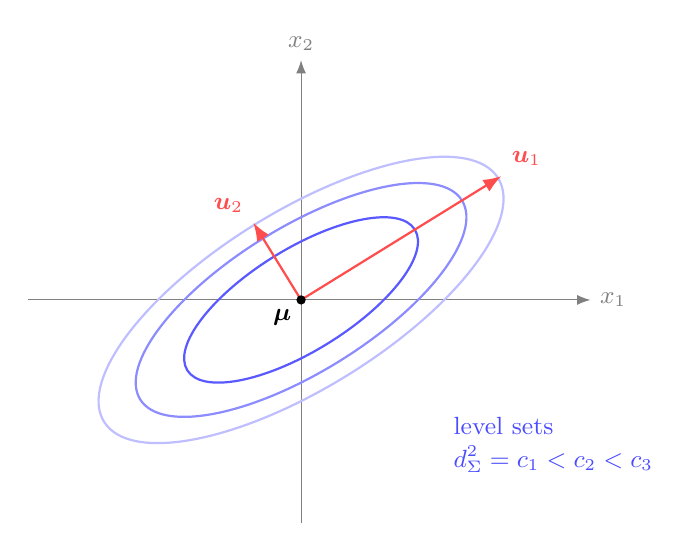
\begin{tikzpicture}[scale=1.05,>=Latex]
    \def\ang{31.72}
    \draw[->,gray] (-3.3,0) -- (3.5,0) node[right]{\small$x_1$};
    \draw[->,gray] (0,-2.7) -- (0,2.9) node[above]{\small$x_2$};
    \begin{scope}[rotate around={\ang:(0,0)}]
        \draw[thick,blue!65] (0,0) ellipse (1.618 and 0.618);
        \draw[thick,blue!45] (0,0) ellipse (2.288 and 0.874);
        \draw[thick,blue!25] (0,0) ellipse (2.802 and 1.070);
        \draw[->,red!70,thick] (0,0) -- (2.85,0) node[above right]{\small$\bu_1$};
        \draw[->,red!70,thick] (0,0) -- (0,1.10) node[above left]{\small$\bu_2$};
    \end{scope}
    \fill (0,0) circle (1.6pt) node[below left]{\small$\bmu$};
    \node[blue!70,align=left] at (3.05,-1.75) {\small level sets\\ \small$d_\Sigma^2=c_1<c_2<c_3$};
\end{tikzpicture}
\caption{Equal-density contours of a bivariate elliptical density with $\bSigma=\left(\begin{smallmatrix}2&1\\1&1\end{smallmatrix}\right)$ (eigenvalues $2.618$ and $0.382$, principal axis at $31.7^\circ$). All contours are homothetic ellipsoids centred at $\bmu$; only their common scale changes with the level, never their shape or orientation.}
\end{figure}

Three readings of the contours:
\begin{enumerate}
    \item \emph{One shape, many levels.} All level sets are \emph{homothetic} copies of one another (semi-axes $\propto\sqrt{u_c}$): the correlation structure fixes the shape and orientation, and the radial profile $g$ fixes only how fast the density decays from the center to the tails. The elliptical family therefore separates ``shape'' (from $\bSigma$) from ``tail thickness'' (from $\psi$).
    \item \emph{Mahalanobis geometry.} $f_{\bX}$ is constant on the sets of constant Mahalanobis distance, so the model treats every direction in the $\bSigma$-metric symmetrically: a shock of given Mahalanobis size is equally likely in every direction. Equivalently, after the linear change of variables $\bz=\bSigma^{-1/2}(\bx-\bmu)$ the contours become spheres, which is the ``spherical in disguise'' content of the definition.
    \item \emph{Financial interpretation and its cost.} Contours of equal joint likelihood being ellipses means that joint crashes and joint rallies are equally likely, and that the probability of a joint move is governed only by the (scalar) distance from the center --- the scalar $R$ is a common ``market factor''. Diversification is thus described entirely by the geometry of $\bSigma$, at the price of excluding exactly the asymmetric, one-sided joint tail events that dominate portfolio losses in practice (see part (e)).
\end{enumerate}

\HWsubproblem
\noindent\textit{Let $L_i=\blambda_i^\top\bX$. Show that}
\[
    \VaR_\alpha(L_i)=\blambda_i^\top\bmu+\sqrt{\blambda_i^\top\bSigma\blambda_i}\,q_\alpha ,
\]
\textit{where $q_\alpha$ is the $\alpha$-quantile of the standardized univariate elliptical distribution.}

\medskip
\textbf{Solution.} By part (a), $L_i\sim E_1\bigl(m_i,s_i^2,\psi\bigr)$ with $m_i=\blambda_i^\top\bmu$ and $s_i^2=\blambda_i^\top\bSigma\blambda_i\ge0$. By the definition used for $\VaR$ in this course, $\VaR_\alpha(L_i)=F_{L_i}^{\leftarrow}(\alpha)$ for $\alpha\in(0,1)$.

Let $Z\sim E_1(0,1,\psi)$ be the standardized univariate elliptical variable, i.e.\ $Z\overset{d}{=}RS_1$ with $R\inde S_1$ and $S_1$ uniform on $\{\pm1\}$, and let $q_\alpha:=F_Z^{\leftarrow}(\alpha)$. If $s_i>0$, then $L_i\overset{d}{=}m_i+s_iZ$ (part (a) with the representation), so $F_{L_i}(x)=\P(Z\le (x-m_i)/s_i)=F_Z((x-m_i)/s_i)$ and, since $x\mapsto(x-m_i)/s_i$ is strictly increasing,
\[
    F_{L_i}^{\leftarrow}(\alpha)=m_i+s_iF_Z^{\leftarrow}(\alpha)=m_i+s_iq_\alpha .
\]
If $s_i=0$, then $L_i=m_i$ a.s.\ and the formula gives $m_i$ as well. Hence
\[
    \boxed{\;\VaR_\alpha(L_i)=\blambda_i^\top\bmu+\sqrt{\blambda_i^\top\bSigma\blambda_i}\,q_\alpha .\;}
\]
\qed

\smallskip
\noindent\textbf{Remark 10.2.} Since $Z\overset{d}{=}-Z$, the law of $Z$ is symmetric about $0$ and $F_Z(0)\ge\frac12$; consequently $q_\alpha\ge0$ for $\alpha\ge\frac12$, which is the key monotonicity used in part (d). The quantity $q_\alpha$ is distribution-free within the family: it depends only on $\psi$ and $\alpha$, not on $\bmu$, $\bSigma$ or the portfolio. For the Gaussian case $q_\alpha=\Phi^{-1}(\alpha)$ and the formula is the familiar $\VaR_\alpha=\blambda^\top\bmu+\sqrt{\blambda^\top\bSigma\blambda}\Phi^{-1}(\alpha)$ of Homework 1, Problem 3.

\HWsubproblem
\noindent\textit{For $\alpha\ge0.5$, prove that}
\[
    \VaR_\alpha\Bigl(\sum_{i=1}^m L_i\Bigr)\le\sum_{i=1}^m\VaR_\alpha(L_i).
\]

\medskip
\textbf{Proof.} Let $\blambda:=\sum_{i=1}^m\blambda_i$, so that $\sum_{i=1}^m L_i=\blambda^\top\bX$. By part (c) applied to $\blambda$ and to each $\blambda_i$,
\begin{equation}\label{eq:dsum}
    \VaR_\alpha\Bigl(\sum_{i=1}^m L_i\Bigr)-\sum_{i=1}^m\VaR_\alpha(L_i)
    =\Bigl(\sqrt{\blambda^\top\bSigma\blambda}-\sum_{i=1}^m\sqrt{\blambda_i^\top\bSigma\blambda_i}\Bigr)q_\alpha ,
\end{equation}
because the location terms cancel: $\blambda^\top\bmu=\sum_i\blambda_i^\top\bmu$.

Since $\bSigma$ is symmetric positive semidefinite, it has a symmetric positive semidefinite square root $\bSigma^{1/2}$ (spectral decomposition), and
\[
    \sqrt{\blambda^\top\bSigma\blambda}=\bigl\|\bSigma^{1/2}\blambda\bigr\|,\qquad
    \sqrt{\blambda_i^\top\bSigma\blambda_i}=\bigl\|\bSigma^{1/2}\blambda_i\bigr\| .
\]
The triangle inequality in $\real^d$ gives
\[
    \Bigl\|\bSigma^{1/2}\sum_{i=1}^m\blambda_i\Bigr\|
    =\Bigl\|\sum_{i=1}^m\bSigma^{1/2}\blambda_i\Bigr\|
    \le\sum_{i=1}^m\bigl\|\bSigma^{1/2}\blambda_i\bigr\|,
\]
so the bracket in \eqref{eq:dsum} is nonpositive. Finally, for $\alpha\ge0.5$ we have $q_\alpha\ge0$ by the symmetry of $Z$ (Remark 10.2), so the product in \eqref{eq:dsum} is $\le0$, i.e.
\[
    \boxed{\;\VaR_\alpha\Bigl(\sum_{i=1}^m L_i\Bigr)\le\sum_{i=1}^m\VaR_\alpha(L_i).\;}
\]
\qed

\smallskip
\noindent\textbf{Remark 10.3.} \emph{(i) Where each hypothesis is used.} Positive semidefiniteness of $\bSigma$ gives the existence of $\bSigma^{1/2}$ and hence subadditivity of $\blambda\mapsto\sqrt{\blambda^\top\bSigma\blambda}$ (a seminorm); $\alpha\ge\frac12$ gives the sign $q_\alpha\ge0$; the common generator $\psi$ makes the \emph{same} $q_\alpha$ appear in every term, which is what allows the location terms to cancel and the scalars to be compared. Drop any one of the three and the inequality can fail --- e.g.\ for a skewed loss distribution VaR can be superadditive, as in Homework 1, Problems 6 and 7 (the Pareto and the skewness counterexamples).

\emph{(ii) Equality.} Equality holds if and only if the vectors $\bSigma^{1/2}\blambda_i$ are parallel and point in the same direction (or $q_\alpha=0$): in that case the ``portfolio'' is a single risk factor in disguise, and no diversification is possible. Otherwise the inequality is strict, and the gap is a genuine diversification benefit measured in the $\bSigma$-metric.

\emph{(iii) $\alpha<\frac12$.} Then $q_\alpha\le0$ and the inequality reverses, $\VaR_\alpha(\sum_iL_i)\ge\sum_i\VaR_\alpha(L_i)$. This is not a paradox: for $\alpha<\frac12$ the $\VaR$ is a quantile in the \emph{gain} part of the distribution, and the reversal reflects that the ``risk'' being measured is then a lower quantile of the P\&L.

\emph{(iv) The same conclusion holds for ES}, with no restriction on $\alpha$: by the coherence of ES (Homework 1, Problem 1) subadditivity holds for every law, elliptical or not.

\HWsubproblem
\noindent\textit{Discuss two advantages and two limitations of elliptical models for financial risk-factor returns.}

\medskip
\textbf{Discussion.}

\smallskip
\noindent\textbf{Two advantages.}
\begin{enumerate}
    \item \emph{Closure under linear aggregation and explicit portfolio risk.} By Problems 7 and 10(a)--(c), every linear portfolio of elliptically distributed risk factors is again elliptical \emph{with the same generator}, and its $\VaR$ (and, by the analogue of part (c) for ES, its ES) is available in closed form from $(\bmu,\bSigma,\psi)$:
    \[
        \VaR_\alpha(\bw^\top\bX)=\bw^\top\bmu+\sqrt{\bw^\top\bSigma\bw}\,q_\alpha,\qquad
        \frac{\partial\VaR_\alpha}{\partial\bw}=\bmu+q_\alpha\frac{\bSigma\bw}{\sqrt{\bw^\top\bSigma\bw}} .
    \]
    Hence no simulation or historical resampling is needed for any portfolio, risk budgeting and Euler risk decomposition are exact and driven by $\bSigma$ alone, and by part (d) $\VaR$ is subadditive for $\alpha\ge\frac12$, so diversification is always rewarded --- the opposite of the skewness counterexample of Homework 1. A further dividend is that the mean--variance frontier is the same for \emph{all} elliptical laws with finite variance, so portfolio selection can be separated from the choice of $\psi$.
    \item \emph{Parsimony with tail flexibility.} The model has only three building blocks $(\bmu,\bSigma,\psi)$, yet $\psi$ can reproduce very different tail behaviour (normal, Student-$t$, Laplace, Cauchy, stable, normal-variance mixtures) and hence match empirically observed $\ES/\VaR$ ratios without extra parameters. Estimation is quasi-maximum-likelihood: $\hat\bmu$ and $\hat\bSigma$ are consistent under ellipticality for a wide class of $\psi$, so the scatter matrix can be estimated robustly (e.g.\ by Kendall's tau or by M-estimators) even when fourth moments do not exist, and scenario generation (simulate $R$, then $\bmu+R\bA\bS$) is cheap and reproducible.
\end{enumerate}

\smallskip
\noindent\textbf{Two limitations.}
\begin{enumerate}
    \item \emph{Symmetry.} An elliptical law satisfies $\bX-\bmu\overset{d}{=}-(\bX-\bmu)$, so gains and losses of equal Mahalanobis size are equally likely, and by part (c) $\VaR_\alpha$ and $\VaR_{1-\alpha}$ are mirror images of each other. Financial return data are markedly asymmetric: equity returns are negatively skewed with a loss tail much heavier than the gain tail, long option positions and credit exposures have strongly one-sided payoffs, and liquidity/peg risk is one-sided. The loss tail is therefore systematically understated (and the gain tail overstated) whenever the true law is skewed, and no extra factors inside $\bSigma$ repair this: asymmetry is a property of $\psi$, not of the covariance.
    \item \emph{A single common mixing variable, hence no idiosyncratic tail and no tail diversification.} In the representation $\bX=\bmu+R\bA\bS$ the same $R$ scales \emph{every} component, so the pairwise tail dependence coefficient is a fixed function of the pairwise correlation alone (zero in the Gaussian case, and identical for every pair with the same correlation), the model cannot produce a large loss in one factor while the others are quiet, and, as noted in Remark 7.1, the far tail of any portfolio is just a rescaled copy of the far tail of $R$: $\ES_\alpha/\VaR_\alpha\to$ a constant independent of the portfolio as $\alpha\uparrow1$. Empirically, diversification benefits do weaken in the tail, but not to the point of a single common tail index; and a portfolio of many names should show a tail that is thinner than any single name's, which a common-$R$ model cannot deliver. Consistently, the elliptical class is not closed under addition of independent heterogeneous factors --- only under linear maps --- so aggregating sub-portfolios with different generators already takes the model outside the family.
\end{enumerate}

\smallskip
\noindent\textbf{Remark 10.4.} A practical middle ground, and the reason parts (a)--(d) remain the workhorse of risk management, is to keep the elliptical machinery for the ``shape'' of risk and to add asymmetry explicitly: a skewed generator (skewed-$t$, generalized hyperbolic) or a copula overlay on the radial part $R$. Formulas of part (c) survive any such change; only the subadditivity argument of part (d), which needs a common symmetric $q_\alpha$, does not.

\end{document}
